\documentclass[../main.tex]{subfiles}
\begin{document}

\section{Solide en 3D}
\subsection{Position d'un solide}
Un solide est définit comme un ensemble de points dont les distances entre chaques points est fixe. 

  % Pour décrire entière entièrement un solide il faut 6 variables.  
  % \subsubsection{Description de la position par rapport à 3 points du solide }
  %   on considère 3 points 
\subsubsection{Angles d'Euler}
\begin{center}
  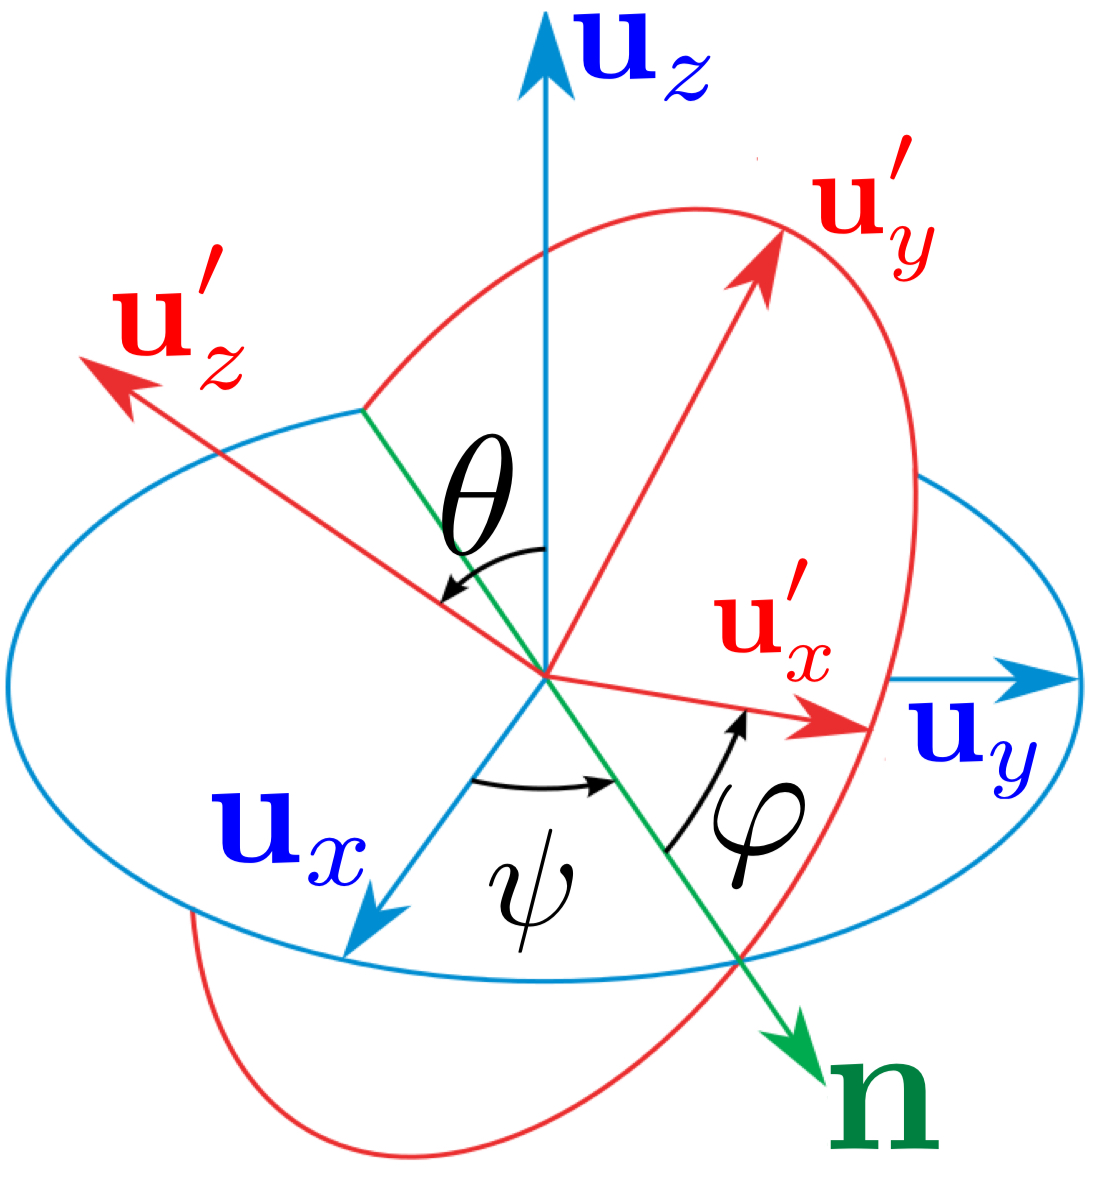
\includegraphics[width=0.07\textwidth]{images/euler.PNG}
\end{center}

Pour passer de \(\refe\) à \(\refe'\) : 
\begin{enumerate}
  \item Précéssion : rotation \(\psi\) autour de \(\uz\) pour amener \(\ux\) sur \(\nod\)
  \item Nutation : rotation \(\theta\) autour de \(\nod\), amène \(\uz\) sur \(\uz'\) 
  \item Rotation propre : rotation \(\varphi\) autour de \(\uz'\), amène \(\nod\) sur \(\ux'\) 
\end{enumerate}

\subsubsection{Vitesse et acceleration d'un point du solide}
\[\vi_p=\vi_{O'}+\vian\times\vv{O'P}\]
\[\ac_p=\ac_{O'}+\diff{\vian}{t}\times\vv{O'P}+\vian\times(\vian\times\vv{O'P})\]

En utilisant un repère cylindrique on on peut dire que \(\vian\times\vv{O'P}=r\diff{\theta}{t}\utheta\) 

On remarque aussi que \(\vian = \dot{\psi}\uz + \dot{\theta}\nod + \dot{\varphi}\uz'\)

\subsubsection{Dynamique d'un corps solide}
\begin{itemize}
  \item Thm du centre de masse : \( M\ac_G = \F^{\exte} \)
  \item Thm du moment cinétique : 
    \begin{enumerate}
      \item \(\diff{\mc_O}{t} = \mf_O^{\exte}\) (\(O\) doit être fixe)
      \item \(\diff{\mc_G}{t} = \mf_G^{\exte}\)
    \end{enumerate} 
  \item Equation de l'énergie : \(\Delta K = W^{\exte}\)
\end{itemize}

\subsection{Rotation autour d'un axe de symétrie \(\Delta_G\)}
\[
  \exists \Delta_G \Leftrightarrow \forall P_i, \exists P_i' \text{ tq. } 
  \begin{cases}
    \vv{GP}_{i\parallel}=\vv{GP}_{i\parallel}'\\
    \vv{GP}_{i\bot}=-\vv{GP}_{i\bot}'\\
  \end{cases}
\]

\subsubsection{Moment cinétique}
Valable seulement autour d'un axe de symétrie : 
\[
  \diff{\mc_G}{t} = \diff{}{t}(I_{\Delta G}\vian)=\mf^{\exte}_G
\]
\subsubsection{Energie cinétique}
\[
  K = K_c + K_r = \tfrac{1}{2}Mv_G^2 + \tfrac{1}{2}I_{\Delta_G}\omega^2
\]

\subsection{Rotation autour d'un axe instantané fixe (=sans vitesse) \(\Delta \parallel \Delta_G\)}
\(O\) est la projection de \(G\) sur \(\Delta\).

Théorème de Huygens-Steiner : 
\[
  I_{\Delta} = Md^2 + I_{\Delta_G}
\]
\[
  \diff{\mc_O}{t} = \diff{}{t}(I_{\Delta}\vian) = I_{\Delta}\diff{\vian}{t}=\mf_O^{\exte}
\]

\textbf{Roulement sans glissement : } vitesse instantané du point de contact est égale à 0, malgré le fait que le point de contact change (+ force de frottement statique).

\end{document}
